\section{Binary search}
\begin{itemize}
    \item Before, we have seen the linear search algorithm which traverses an array, of which worse case complexity was $O(n)$.
    \item In case of binary search, the worse case complexity is narrowed down to $O(\log_{}\p{ n } )$.
    \item Now this algorithm works for looking for target data in a list or array, the array has to be in sorted order, ascending or decending order, but in order.
    \item Binary search is best applied when the elements are kept in a binary search tree. 
    \item For a binary search tree no overhead is here for keeping the elements in sorted order. 
    \item The list or array must be in order, ascending or descending, but in order. 
\end{itemize}

\subsection{Example}
\begin{itemize}
    \item Consider variables lower bound and upper bound, these hold the current bounds in which the array will be searched. Suppose we want to find 59 in the list.
\end{itemize}

\subsection{Searching the upper part}
\begin{figure}[H]
    \centering
    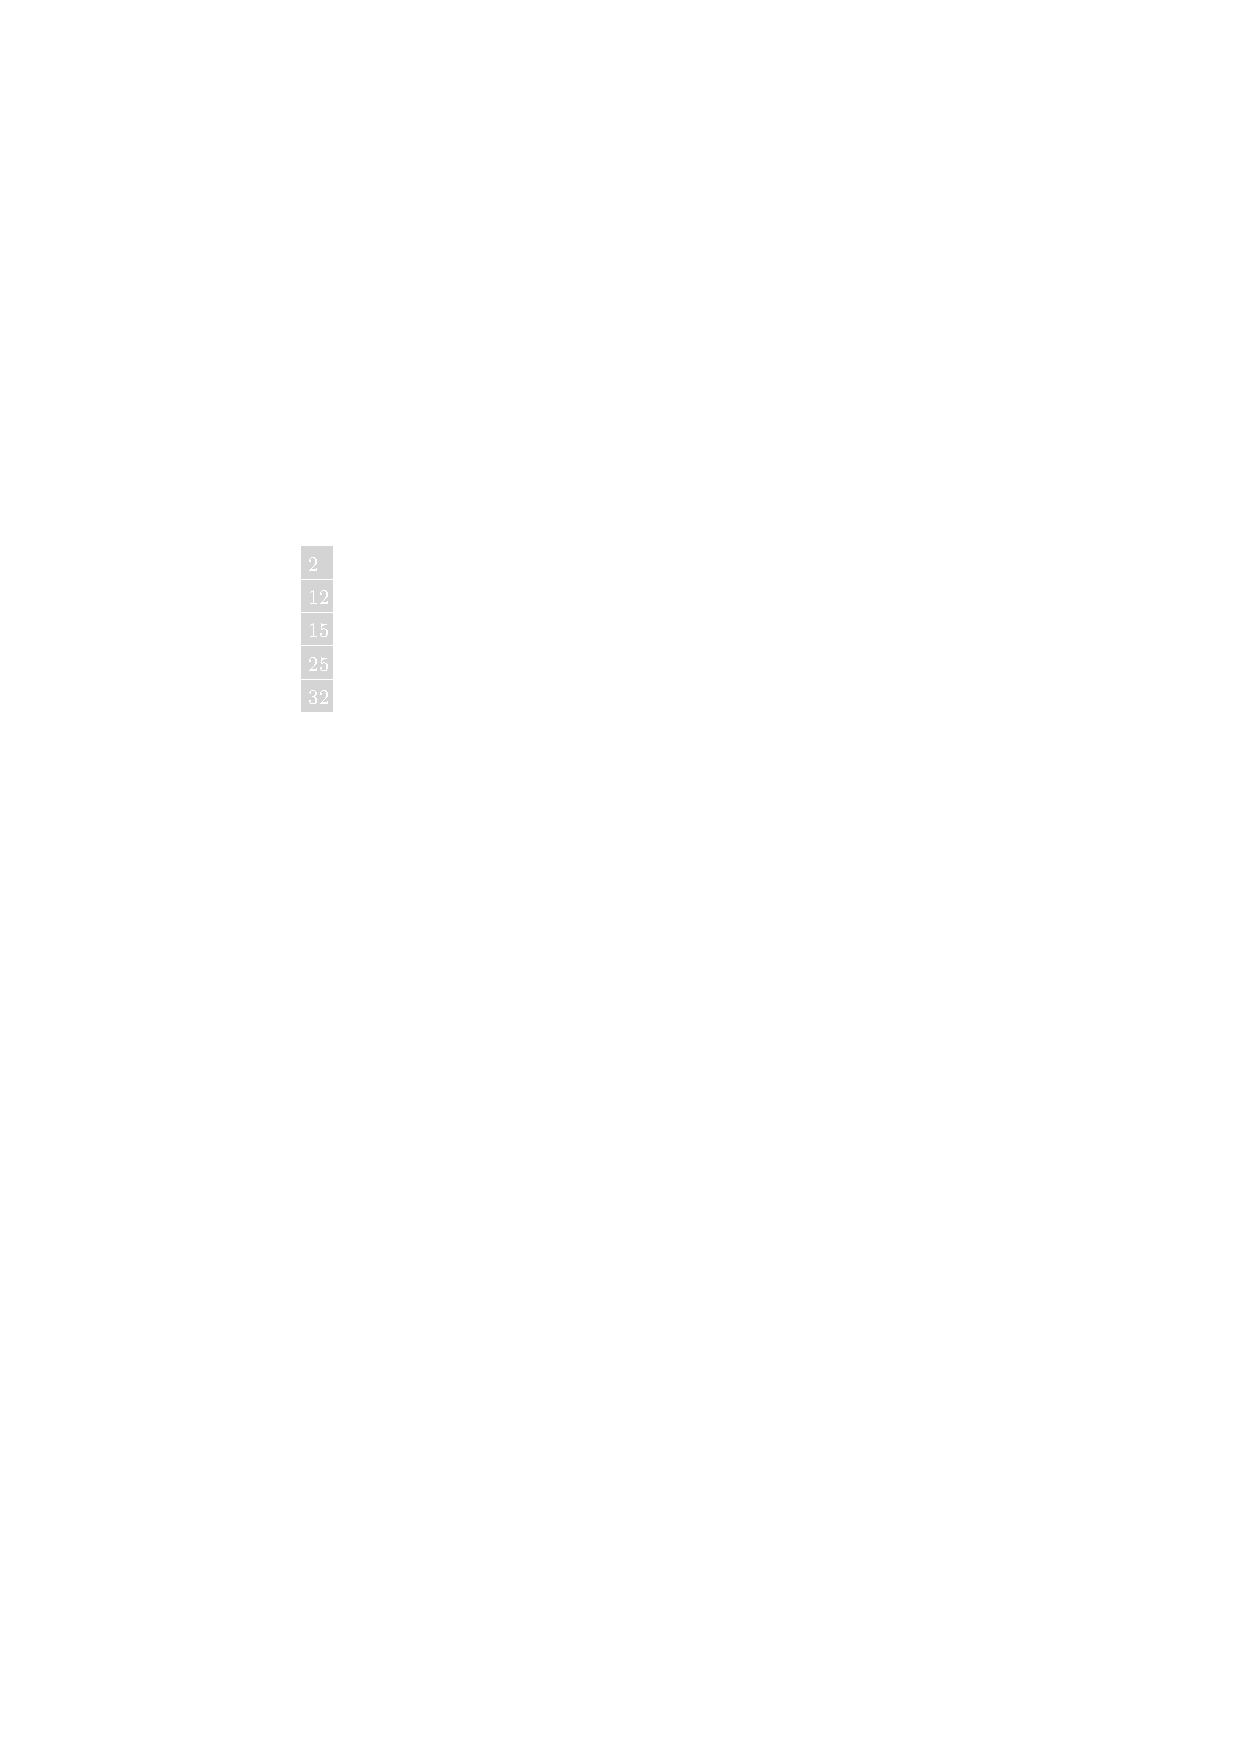
\includegraphics[]{\figs/binarysearch}
\end{figure}

\subsection{Searching the lower part}
\begin{figure}[H]
    \centering
    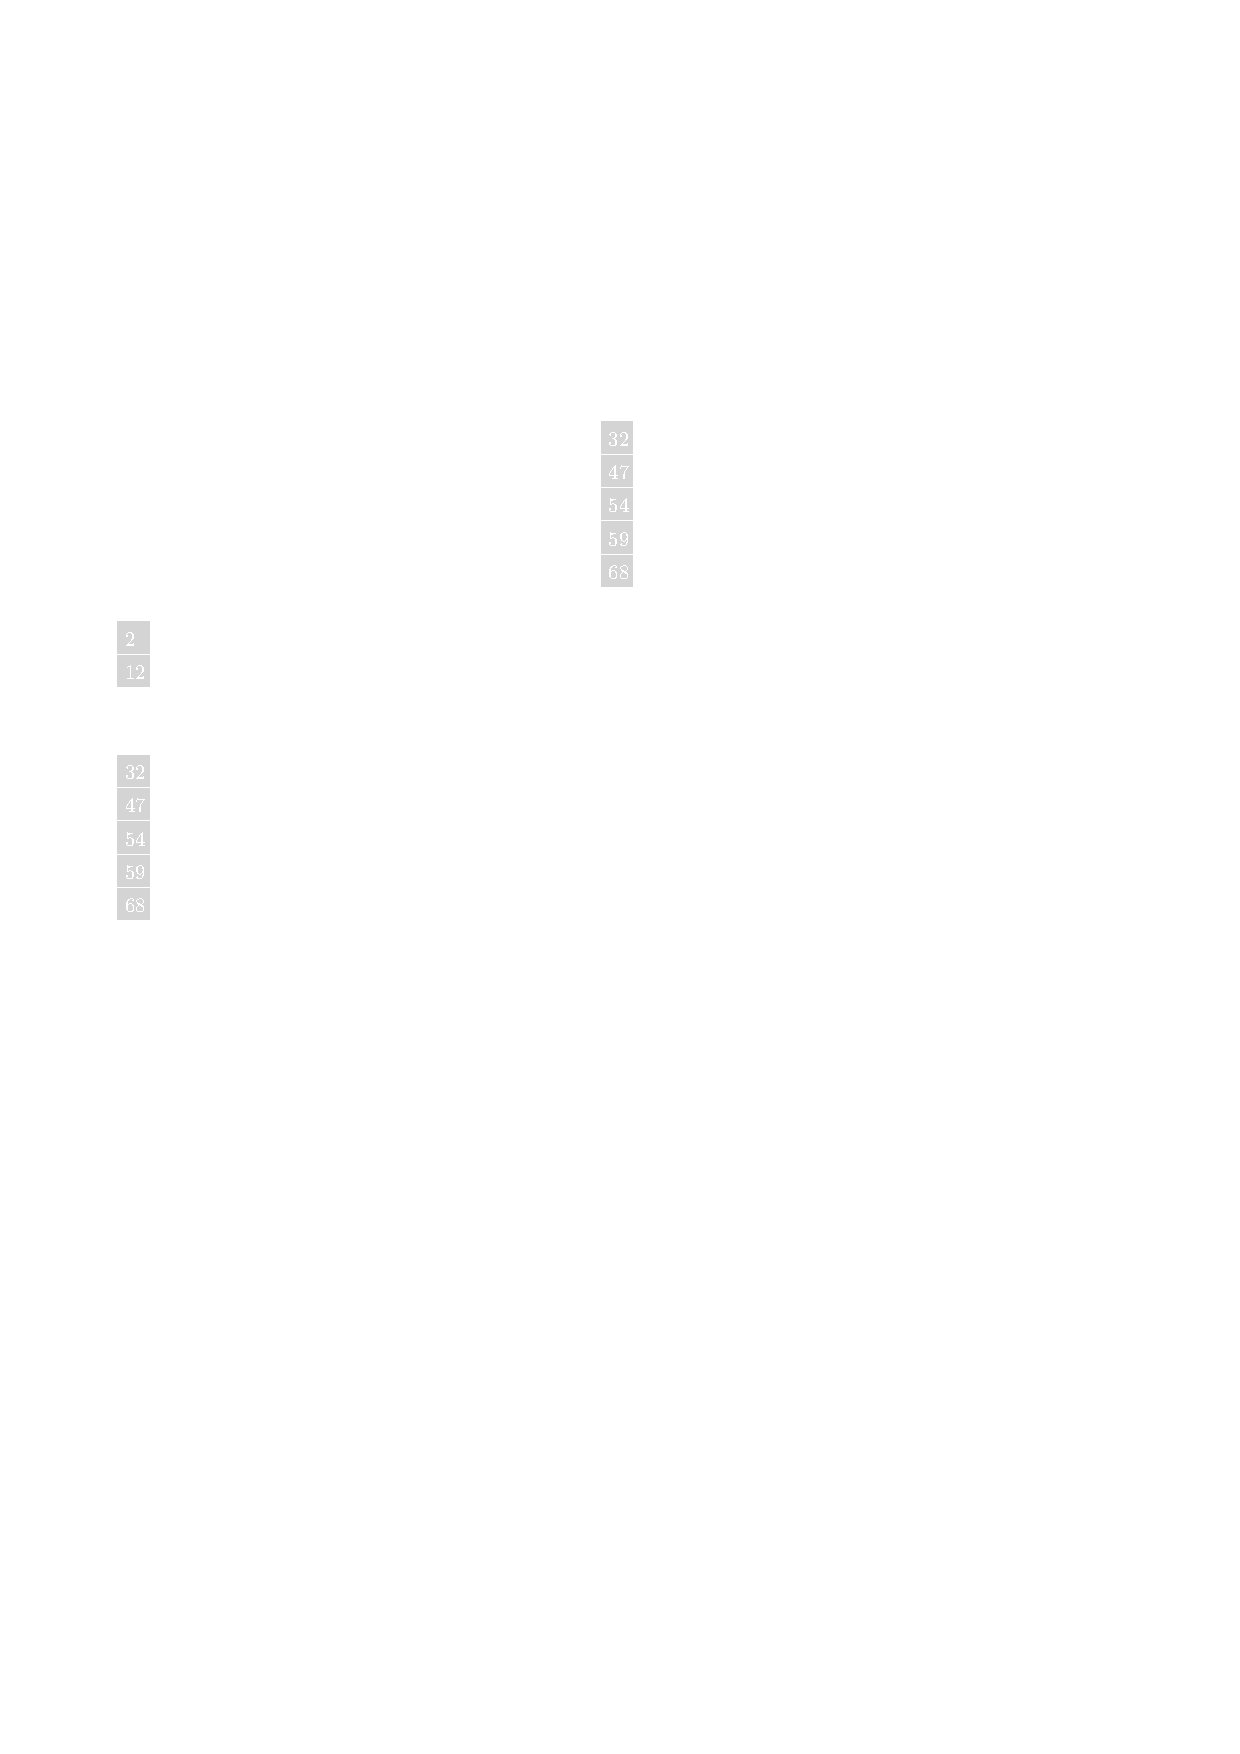
\includegraphics[]{\figs/binarysearch1} 
\end{figure}

\subsection{When the target is not on the list}
\begin{figure}[H]
    \centering
    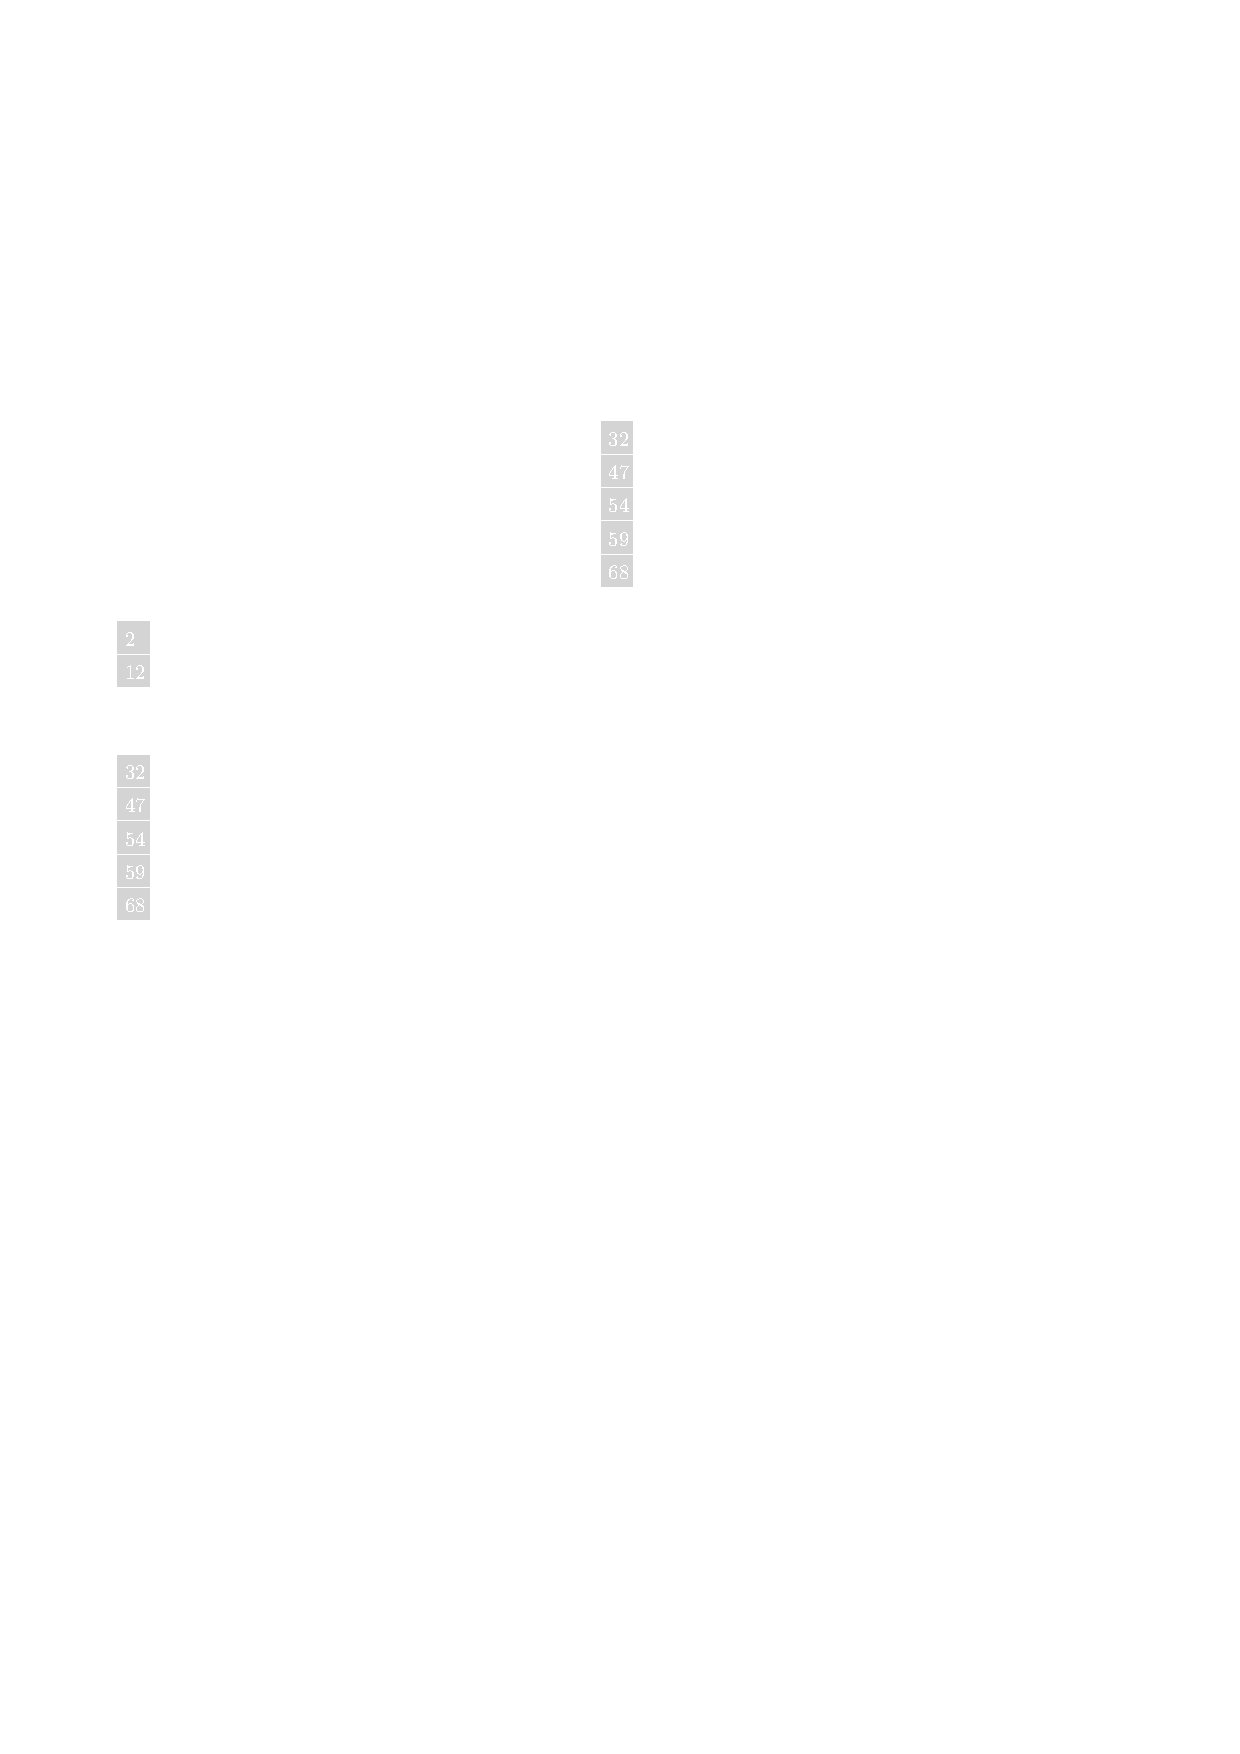
\includegraphics[]{\figs/binarysearch1} 
\end{figure}

\section{Implementation}
\inputcode{c}{\code/binary_search.c}

\section{Worst case complexity}
On each iteration the $n$ is split in two, $n \rightarrow n/2 \rightarrow n / 2^2$ and eventually we'll get to $n/2^i = n / n = 1$ this will happen when $i = \log_{2}\p{ n } $ there is only one comparison happening in each iteration because of the if,else if and else; since this is the case there are $\log_{}\p{n}$ comparisons. Thus, the Big-O is $O(\log_{}\p{ n } )$.
